% ============================================================
% Beamer — ISLP Lecture Series — IMPROVED EDITION
% Advanced Module A12: Bayesian Inference
% ============================================================
\documentclass[aspectratio=169,11pt]{beamer}
\usepackage[utf8]{inputenc}\usepackage[T1]{fontenc}\usepackage[english]{babel}
\usepackage{graphicx}\usepackage{booktabs}\usepackage{amsmath,amssymb,amsfonts}
\usepackage{mathtools}\usepackage{hyperref}\usepackage{xcolor}
\usepackage{verbatim}\usepackage{alltt}
\usepackage{tikz}\usetikzlibrary{calc,arrows.meta,positioning,shapes}
\usepackage{tcolorbox}\tcbuselibrary{skins}

\usetheme{Madrid}\usecolortheme{default}
\setbeamertemplate{navigation symbols}{}
\setbeamertemplate{footline}[frame number]
\setbeamertemplate{blocks}[rounded][shadow=false]
\setbeamertemplate{headline}{%
  \leavevmode\hbox{%
    \begin{beamercolorbox}[wd=\paperwidth,ht=2.2ex,dp=0.9ex]{section in head/foot}%
      {\fontsize{4.6}{5.2}\selectfont%
       \insertsectionnavigationhorizontal{\paperwidth}{}{\hskip0pt plus1filll}}%
    \end{beamercolorbox}}%
}
\setbeamerfont{section in head/foot}{size=\tiny}
\setbeamerfont{palette primary}{size=\tiny}
\setbeamerfont{palette tertiary}{size=\tiny}
\setbeamerfont{section in toc}{size=\footnotesize}

\usepackage{listings}
\definecolor{pyKw}{RGB}{0,0,180}\definecolor{pyStr}{RGB}{20,120,40}
\definecolor{pyCom}{RGB}{120,120,120}\definecolor{accent}{RGB}{38,70,140}
\lstdefinestyle{Pystyle}{language=Python,basicstyle=\ttfamily\footnotesize,
  keywordstyle=\color{pyKw}\bfseries,commentstyle=\color{pyCom}\itshape,
  stringstyle=\color{pyStr},showstringspaces=false,upquote=true,
  columns=fullflexible,breaklines=true,literate={~}{{$\sim$}}1}
\lstset{style=Pystyle}

% Tighter TOC spacing (place AFTER \lstset, BEFORE \AtBeginSection)
\usepackage{etoolbox}
\makeatletter
\patchcmd{\beamer@sectionintoc}{\vskip1.5em}{\vskip.6em}{\typeout{TOCPATCH-OK}}{\typeout{TOCPATCH-FAIL}}
\makeatother

\AtBeginSection[]{\begin{frame}{Outline}\footnotesize
  \tableofcontents[currentsection,sectionstyle=show/shaded,subsectionstyle=show/show/hide]
\end{frame}}

\newcommand{\islpsource}[1]{%
  \vfill\hfill{\tiny\itshape\color{gray}Source: #1 \textemdash{} ISLP, James et al.\ (2023).}\par
}

\newtcolorbox{takeaway}[1][Takeaway]{enhanced,colback=green!4,colframe=green!50!black,
  boxrule=0pt,leftrule=2.5pt,arc=2pt,fonttitle=\bfseries,title=#1,
  left=2mm,right=2mm,top=1mm,bottom=1mm}
\newtcolorbox{numexample}[1][Worked example]{enhanced,colback=orange!4,colframe=orange!70!black,
  boxrule=0pt,leftrule=2.5pt,arc=2pt,fonttitle=\bfseries,title=#1,
  left=2mm,right=2mm,top=1mm,bottom=1mm}
\newtcolorbox{readme}[1][How to read this]{enhanced,colback=blue!4,colframe=accent,
  boxrule=0pt,leftrule=2.5pt,arc=2pt,fonttitle=\bfseries,title=#1,
  left=2mm,right=2mm,top=1mm,bottom=1mm}

\title{Quantitative Research Methods}
\subtitle{Bayesian Inference\\[2pt]{\small Advanced module A12 --- optional self-study}}
\author{Prof.\ Dr.\ Christoph Weisser}
\date{}\graphicspath{{images/}}

\newtcolorbox{exercise}[1][Exercise]{enhanced, fontupper=\footnotesize, colback=purple!4, colframe=purple!55!black, boxrule=0pt, leftrule=2.5pt, arc=2pt, fonttitle=\bfseries, title=#1, left=2mm, right=2mm, top=1mm, bottom=1mm}
\newtcolorbox{solutionbox}[1][Solution]{enhanced, colback=teal!5, colframe=teal!55!black, boxrule=0pt, leftrule=2.5pt, arc=2pt, fonttitle=\bfseries, title=#1, left=2mm, right=2mm, top=1mm, bottom=1mm}
\newtcolorbox{longexercise}[1][Extended exercise (15 min)]{enhanced, fontupper=\footnotesize, colback=violet!6, colframe=violet!55!black, boxrule=0pt, leftrule=3pt, arc=2pt, fonttitle=\bfseries, title=#1, left=2mm, right=2mm, top=1mm, bottom=1mm}

% Reclaim ~2pt of body height (custom nav headline makes full slides tip over by ~1.83pt)
\addtobeamertemplate{frametitle}{}{\vspace{-2pt}}

\newtcolorbox{labnote}[1][Run this live in the lab notebook]{enhanced, fontupper=\footnotesize, colback=cyan!7, colframe=cyan!45!black, boxrule=0pt, leftrule=3pt, arc=2pt, fonttitle=\bfseries, title=#1, left=2mm, right=2mm, top=1mm, bottom=1mm}

% Common-mistake callout --- crimson, for the error to pre-empt
\newtcolorbox{mistake}[1][Common mistake]{enhanced, fontupper=\footnotesize, colback=red!4, colframe=red!60!black, boxrule=0pt, leftrule=3pt, arc=2pt, fonttitle=\bfseries, title=#1, left=2mm, right=2mm, top=1mm, bottom=1mm}

\begin{document}
\begin{frame}[plain]\titlepage\end{frame}

\begin{frame}{Where this module fits}
  \footnotesize
  \begin{center}
  \begin{tabular}{@{}p{3.9cm}p{8.4cm}@{}}
    \toprule
    \textbf{Course chapter / module} & \textbf{What this module builds on it} \\
    \midrule
    Ch.\ 0 --- statistics refresher & Confidence intervals and $p$-values --- here they get rivals \\
    Ch.\ 3 --- linear regression & The likelihood; Bayesian regression reuses the whole fit \\
    Ch.\ 4 --- classification & Bayes' theorem itself (LDA already used it for labels) \\
    Ch.\ 6 --- regularisation & Ridge \emph{is} a Bayesian estimate in disguise --- proved here \\
    \bottomrule
  \end{tabular}
  \end{center}
  \vspace{2pt}
  \begin{takeaway}[The other way to be uncertain]
    The whole taught course is frequentist: parameters are fixed, data are random.
    This module flips it --- \textbf{treat the parameter as the random thing},
    update beliefs with data, and read off statements the frequentist machinery
    cannot make: ``the probability that $p$ exceeds $0.25$ is $0.93$.''
  \end{takeaway}
  {\scriptsize One of twelve optional advanced modules; self-study. Every number on
  these slides is reproduced by \texttt{make\_figures.py} in the module folder.}
\end{frame}

\begin{frame}{Contents}\small\tableofcontents[hideallsubsections]
  \vfill
  {\tiny Optional and advanced material is collected in the \textbf{appendix} at the end of the deck.}
\end{frame}

\begin{frame}{Notation in this module}
  \footnotesize
  \begin{center}
  \begin{tabular}{@{}ll@{}}
    \toprule
    \textbf{Symbol} & \textbf{Meaning} \\
    \midrule
    $\theta$ & the unknown parameter, now carrying a distribution \\
    $\pi(\theta)$ & the prior: belief before the data \\
    $L(\theta) = p(\text{data} \mid \theta)$ & the likelihood (Chapters 3--4's object) \\
    $\pi(\theta \mid \text{data})$ & the posterior: belief after the data \\
    $\text{Beta}(a, b)$ & the workhorse prior for a probability \\
    CrI & credible interval (posterior probability interval) \\
    MAP & maximum a posteriori: the posterior's peak \\
    $\tau$ & prior standard deviation (how sure you are beforehand) \\
    \bottomrule
  \end{tabular}
  \end{center}
\end{frame}

\begin{frame}{Sources and references}
  \begin{block}{Primary textbook}
    James, Witten, Hastie, Tibshirani \& Taylor (2023),
    \emph{An Introduction to Statistical Learning, with Applications in Python},
    Springer. --- Supplies the likelihoods, ridge, and the datasets
    (\texttt{Advertising.csv}).
  \end{block}
  \begin{block}{Canonical further reading (optional)}
    Gelman et al., \emph{Bayesian Data Analysis} (3rd ed., 2013);
    McElreath, \emph{Statistical Rethinking} (2nd ed., 2020) --- the standard
    references, one formal, one narrative.
  \end{block}
\end{frame}

\begin{frame}{Learning objectives}
  By the end of this module you will be able to:
  \begin{itemize}
    \item \textbf{State} Bayes' theorem for parameters and the roles of prior,
          likelihood and posterior.
    \item \textbf{Update} a Beta prior with binomial data by hand, and report a
          posterior mean and credible interval.
    \item \textbf{Explain} every posterior mean in this module as a
          \emph{precision-weighted compromise} between prior and data.
    \item \textbf{Derive} ridge regression as the MAP estimate under a Gaussian
          prior --- and translate $\lambda \leftrightarrow \tau$.
    \item \textbf{Implement} a Metropolis sampler from scratch and check it against
          the analytic answer.
    \item \textbf{Distinguish} credible from confidence intervals without garbling
          either.
  \end{itemize}
\end{frame}

\begin{frame}{Roadmap of this module}
  \begin{takeaway}[{{Believe, observe, update}}]
    \begin{enumerate}
      \item The problem: what kind of probability a parameter can have.
      \item The Beta--binomial engine: updating by hand, priors, credible
            intervals.
      \item Gaussian means and shrinkage: precision weighting --- and ridge
            unmasked.
      \item Computation: when conjugacy runs out, walk (Metropolis).
      \item Bayesian regression and decisions: \texttt{Advertising}, and an A/B
            call.
      \item Python lab, summary, appendix.
    \end{enumerate}
  \end{takeaway}
\end{frame}

% ============================================================
\section{The Problem}
% ============================================================

\begin{frame}{Two questions that sound the same}
  \begin{center}
  \footnotesize
  \begin{tabular}{@{}p{5.4cm}p{5.9cm}@{}}
    \toprule
    \textbf{Frequentist (Ch.\ 0)} & \textbf{Bayesian (this module)} \\
    \midrule
    How would my estimate vary across imaginary repeated samples? &
    What should I believe about $\theta$, given the one sample I have? \\
    Parameter fixed, data random & Data fixed, parameter random \\
    $p$-value, confidence interval & posterior, credible interval \\
    ``$95\%$ of such intervals cover'' & ``$95\%$ probability $\theta$ is in here'' \\
    \bottomrule
  \end{tabular}
  \end{center}
  \begin{block}{Rule (Bayes' theorem for parameters)}
    \[
      \boxed{\;\pi(\theta \mid \text{data})
        \;\propto\; L(\theta)\,\pi(\theta)\;}
      \qquad \text{posterior} \propto \text{likelihood} \times \text{prior}.
    \]
  \end{block}
  \begin{readme}[How to read this]
    \footnotesize
    Chapter 4's LDA already ran Bayes' theorem --- on \emph{class labels}. The only
    new move is to run it on \emph{parameters}. The likelihood is the same object
    Chapters 3--4 maximised; the prior is new; the posterior is the answer.
  \end{readme}
\end{frame}

\begin{frame}{Exercise A12.1 --- Credible or confident? [Concept]}
  \begin{exercise}
    A 95\% \emph{confidence} interval for a conversion rate is $[0.19, 0.31]$; a
    95\% \emph{credible} interval from the same data is $[0.19, 0.31]$ as well.
    \begin{enumerate}
      \item Write the one-sentence claim each interval is entitled to make.
      \item A manager says: ``there is a $95\%$ chance the true rate is between
            $0.19$ and $0.31$.'' Which interval licenses that sentence?
      \item Why do the two intervals often nearly coincide anyway?
    \end{enumerate}
  \end{exercise}
\end{frame}

\begin{frame}{Solution --- Exercise A12.1}
  \begin{solutionbox}
    \footnotesize
    \textbf{Part 1.} Confidence: ``this interval was built by a recipe that
    captures the true rate in $95\%$ of repeated samples'' --- a statement about
    the \emph{procedure}. Credible: ``given the data and the prior, the posterior
    probability that the rate lies in $[0.19, 0.31]$ is $0.95$'' --- a statement
    about \emph{this} interval.
    \par\smallskip
    \textbf{Part 2.} Only the credible interval. The manager's sentence assigns a
    probability to the parameter, which frequentist logic forbids: once computed,
    a confidence interval either contains the fixed truth or does not. (Everyone
    reads confidence intervals the manager's way --- Chapter 0 flagged the
    misreading; here it becomes a licensed statement.)
    \par\smallskip
    \textbf{Part 3.} With a flat-ish prior and decent $n$, the posterior is
    essentially the normalised likelihood, so both intervals track the same
    curvature --- they agree numerically while meaning different things. The
    divergence appears when priors are informative or $n$ is small.
  \end{solutionbox}
\end{frame}

% ============================================================
\section{The Beta-Binomial Engine}
% ============================================================

\begin{frame}{Conjugacy: the update you can do in your head}
  \begin{block}{Rule (Beta--binomial conjugacy)}
    \[
      \text{prior } \text{Beta}(a, b)\; +\; y \text{ successes in } n \text{ trials}
      \;\Longrightarrow\;
      \boxed{\;\text{posterior } \text{Beta}(a + y,\; b + n - y)\;}
    \]
  \end{block}
  \begin{readme}[How to read this]
    \footnotesize
    The prior acts like $a + b$ \emph{imaginary trials}, $a$ of them successes.
    Updating is bookkeeping: add real successes to $a$, real failures to $b$.
    Posterior mean $= \frac{a + y}{a + b + n}$ --- always \emph{between} the prior
    mean and the sample proportion.
  \end{readme}
  \begin{numexample}[{{A conversion rate, true $p = 0.3$}}]
    Prior $\text{Beta}(2,2)$. After $n=10$ ($y=2$): $\text{Beta}(4,10)$, mean
    $0.286$. After $n=50$ ($y=12$): $\text{Beta}(14,40)$, mean $0.259$. After
    $n=200$ ($y=49$): $\text{Beta}(51,153)$, mean $0.250$, 95\% CrI
    $[0.193,\, 0.312]$.
  \end{numexample}
\end{frame}

\begin{frame}{Watching belief sharpen}
  \begin{center}
    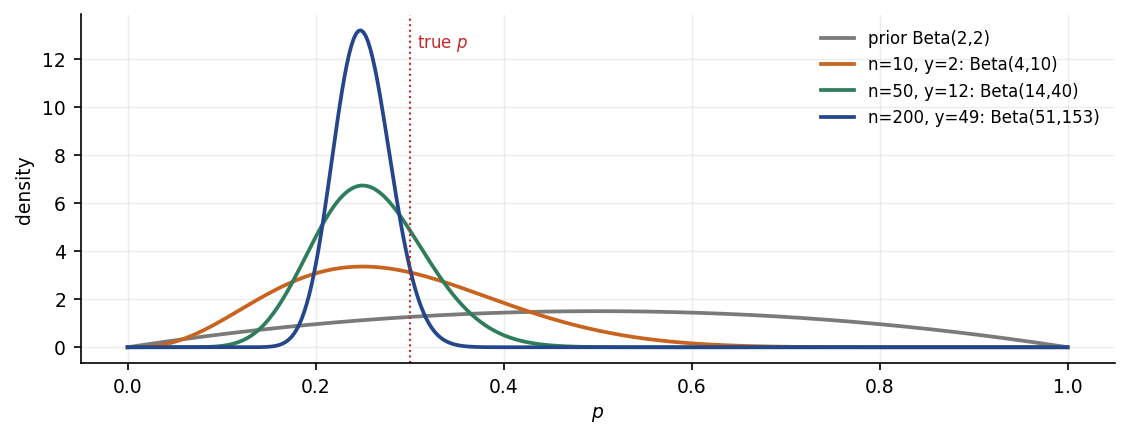
\includegraphics[width=0.86\textwidth,height=0.46\textheight,keepaspectratio]{cha12_beta_update.png}
  \end{center}
  \begin{takeaway}[Data overwhelm the prior --- at the data's own pace]
    \footnotesize
    The gentle $\text{Beta}(2,2)$ hump narrows steadily; by $n = 200$ the posterior
    is tight around the sample rate and the prior's four imaginary trials are
    outvoted $50:1$. The truth ($0.3$) sits inside every credible interval along
    the way.
  \end{takeaway}
\end{frame}

\begin{frame}{Three priors, one dataset}
  \begin{center}
    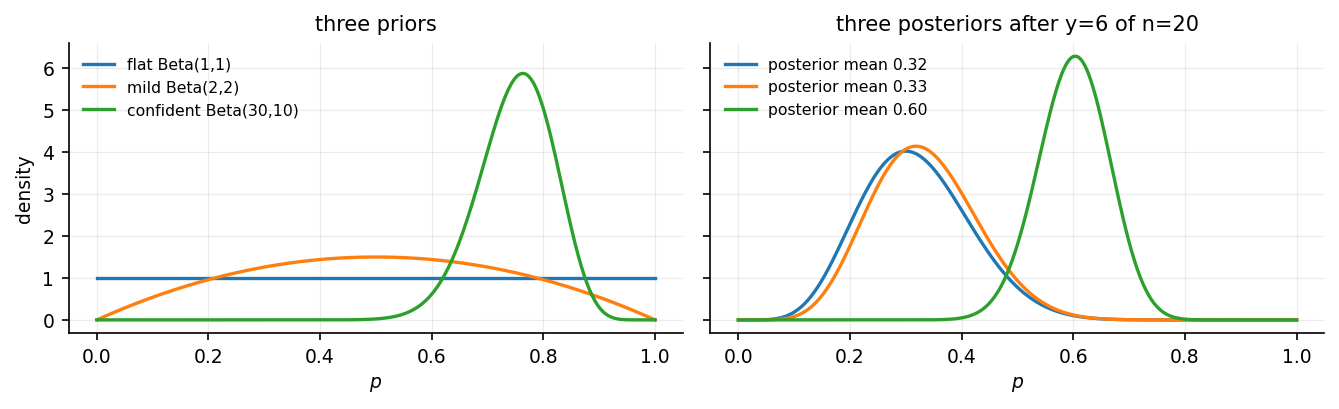
\includegraphics[width=0.9\textwidth,height=0.44\textheight,keepaspectratio]{cha12_priors.png}
  \end{center}
  \begin{takeaway}[{{Priors matter exactly as much as they claim to}}]
    \footnotesize
    Same data ($y = 6$ of $n = 20$). Flat prior $\to$ mean $0.318$; mild
    $\text{Beta}(2,2) \to 0.333$; a confident-but-wrong $\text{Beta}(30,10)$
    (forty imaginary trials at $75\%$) $\to \mathbf{0.600}$ --- the data are
    outvoted $2{:}1$. A prior is a claim with a stake; make it inspectable, and
    show the sensitivity.
  \end{takeaway}
\end{frame}

\begin{frame}{Exercise A12.2 --- One update by hand [Math]}
  \begin{exercise}
    Prior $\text{Beta}(2, 2)$ on a click-through rate; you observe $7$ clicks in
    $10$ impressions.
    \begin{enumerate}
      \item Write down the posterior distribution.
      \item Compute the prior mean, the MLE, and the posterior mean.
      \item Show that the posterior mean is a weighted average
            $w \cdot \text{MLE} + (1 - w) \cdot \text{prior mean}$, and identify
            $w$.
    \end{enumerate}
  \end{exercise}
\end{frame}

\begin{frame}{Solution --- Exercise A12.2}
  \begin{solutionbox}
    \footnotesize
    \textbf{Part 1.} $\text{Beta}(2 + 7,\; 2 + 3) = \text{Beta}(9, 5)$.
    \par\smallskip
    \textbf{Part 2.} Prior mean $= 2/4 = 0.5$; MLE $= 7/10 = 0.7$; posterior mean
    $= 9/14 \approx \mathbf{0.643}$.
    \par\smallskip
    \textbf{Part 3.} With $a + b = 4$ prior trials and $n = 10$ real ones,
    \[
      \frac{a + y}{a + b + n}
        = \underbrace{\frac{n}{n + a + b}}_{w = 10/14}\cdot\frac{y}{n}
        + \underbrace{\frac{a + b}{n + a + b}}_{1 - w = 4/14}\cdot\frac{a}{a+b}
        = \tfrac{10}{14}(0.7) + \tfrac{4}{14}(0.5) = 0.643.
    \]
    The weight on the data is \emph{sample size against imaginary sample size} ---
    the entire prior-vs-data politics of this module in one fraction.
  \end{solutionbox}
  \begin{mistake}
    Reporting the MAP ($8/12 = 0.667$) as ``the Bayesian estimate'' without saying
    so. Mean, median and MAP all summarise the posterior; for skewed posteriors
    they differ, and the honest report is the whole interval.
  \end{mistake}
\end{frame}

% ============================================================
\section{Gaussian Means \& Shrinkage}
% ============================================================

\begin{frame}{The Gaussian mean: precision-weighted compromise}
  \begin{block}{Rule (known $\sigma$, prior $\mu \sim N(\mu_0, \tau^2)$)}
    \[
      \boxed{\;\text{posterior mean}
        = w\,\bar x + (1 - w)\,\mu_0,
      \qquad
      w = \frac{n/\sigma^2}{n/\sigma^2 + 1/\tau^2}\;}
    \]
    posterior variance $= \big(n/\sigma^2 + 1/\tau^2\big)^{-1}$.
  \end{block}
  \begin{readme}[How to read this]
    \footnotesize
    Precisions (inverse variances) \emph{add}; means combine \emph{weighted by
    precision}. The data's vote grows linearly in $n$; the prior's vote is fixed
    --- the Beta--binomial story again, in Gaussian dress.
  \end{readme}
  \begin{numexample}[{{Prior $N(100, 15^2)$, $\sigma = 20$, truth $130$}}]
    \footnotesize
    $n = 2$: mean $105.6$, weight on data $0.53$. $n = 10$: $122.4$, weight
    $0.85$. $n = 50$: $129.5$, weight $0.97$ --- the prior fades on schedule.
  \end{numexample}
\end{frame}

\begin{frame}{The prior fading, drawn}
  \begin{center}
    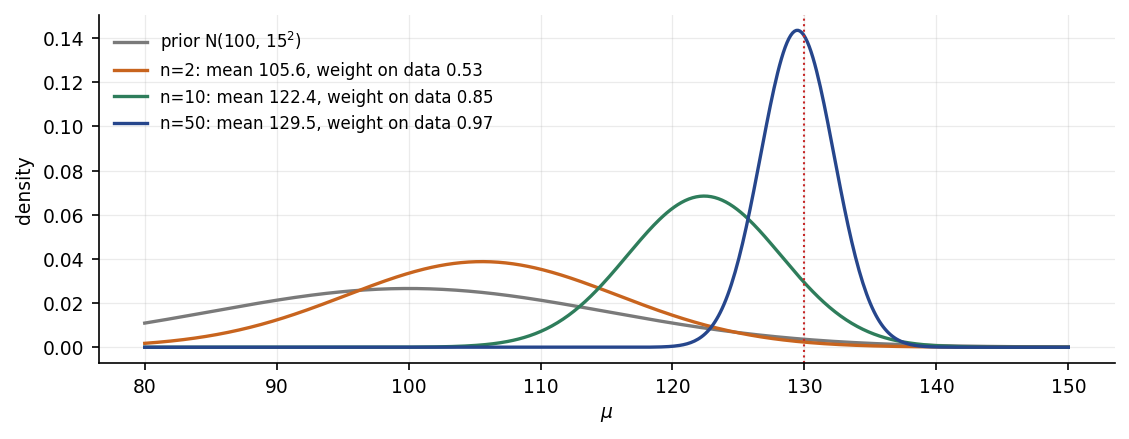
\includegraphics[width=0.86\textwidth,height=0.48\textheight,keepaspectratio]{cha12_gauss_shrink.png}
  \end{center}
  \begin{takeaway}[Shrinkage is not a bug]
    \footnotesize
    At $n = 2$ the posterior barely moves off the prior --- and that is the
    \emph{correct} behaviour: two noisy observations should not overturn a
    considered belief. Every shrinkage estimator in Chapter 6 is this picture
    wearing an optimisation costume, as the next slide proves.
  \end{takeaway}
\end{frame}

\begin{frame}{Ridge regression, unmasked}
  \begin{block}{Claim}
    Ridge (Ch.\ 6) is the \textbf{MAP estimate} of a linear model under the prior
    $\beta_j \sim N(0, \tau^2)$, with
    $\;\boxed{\lambda = \sigma^2 / \tau^2}$.
  \end{block}
  \begin{readme}[The two-line proof]
    \footnotesize
    Maximising the log-posterior $=$ log-likelihood $+$ log-prior:
    \[
      -\tfrac{1}{2\sigma^2}\textstyle\sum_i (y_i - x_i^\top\beta)^2
      \;-\; \tfrac{1}{2\tau^2}\textstyle\sum_j \beta_j^2
      \;\;\propto\;\;
      -\Big[\textstyle\sum_i (y_i - x_i^\top\beta)^2
        + \tfrac{\sigma^2}{\tau^2}\textstyle\sum_j \beta_j^2\Big],
    \]
    which is exactly the ridge criterion with $\lambda = \sigma^2/\tau^2$.
  \end{readme}
  \begin{takeaway}[{{Chapter 6's tuning dial, translated}}]
    \footnotesize
    A large penalty $\lambda$ \emph{is} a tight prior ($\tau$ small).
    Cross-validating $\lambda$ empirically chooses how strong a prior the data
    can support. (The lasso? A Laplace prior --- same construction.)
  \end{takeaway}
\end{frame}

\begin{frame}{The dictionary, drawn on Advertising}
  \begin{center}
    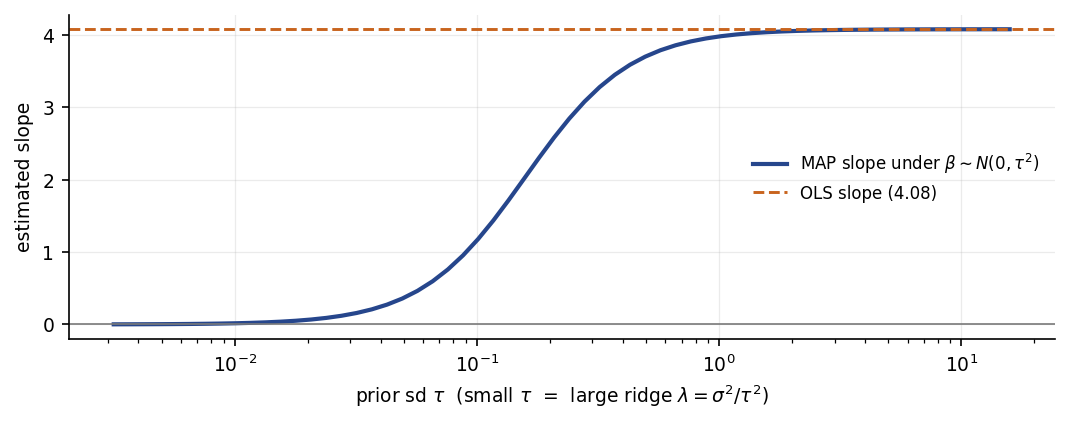
\includegraphics[width=0.82\textwidth,height=0.46\textheight,keepaspectratio]{cha12_ridge_map.png}
  \end{center}
  \begin{takeaway}[Read the dial]
    \footnotesize
    Standardised \texttt{sales}-on-\texttt{TV} slope: OLS says $4.08$. As the prior
    tightens ($\tau \downarrow$), the MAP slope shrinks toward $0$ --- at
    $\tau = 0.1$ (i.e.\ $\lambda = 500$) it is $1.16$. Chapter 6's whole
    coefficient-path figure is this curve, one predictor at a time.
  \end{takeaway}
\end{frame}

\begin{frame}{Exercise A12.3 --- Precision weighting by hand [Math]}
  \begin{exercise}
    Quality control believes a machine fills bottles at $\mu_0 = 100$ml
    ($\tau = 15$). Measurement noise is $\sigma = 20$. A morning sample gives
    $n = 4$, $\bar x = 120$.
    \begin{enumerate}
      \item Compute the posterior mean and standard deviation of $\mu$.
      \item The engineer says ``the sample says 120, so recalibrate to 120.''
            What does the posterior say instead, and why?
      \item How large would $n$ (at $\bar x = 120$) have to be for the weight on
            the data to reach $0.9$?
    \end{enumerate}
  \end{exercise}
\end{frame}

\begin{frame}{Solution --- Exercise A12.3}
  \begin{solutionbox}
    \footnotesize
    \textbf{Part 1.} Precisions: prior $1/\tau^2 = 1/225 \approx 0.00444$;
    data $n/\sigma^2 = 4/400 = 0.01$. Weight on data
    $w = 0.01 / 0.01444 \approx 0.692$. Posterior mean
    $= 0.692 \times 120 + 0.308 \times 100 \approx \mathbf{113.8}$;
    posterior sd $= \sqrt{1/0.01444} \approx \mathbf{8.3}$.
    \par\smallskip
    \textbf{Part 2.} Split the difference toward $113.8$: with only four noisy
    measurements ($\text{SE} = 20/2 = 10$), a $20$ml jump from a well-calibrated
    prior is as likely to be sampling noise as drift. The posterior \emph{is} the
    rational compromise --- and its sd ($8.3$) says a follow-up sample is worth
    taking before touching the machine.
    \par\smallskip
    \textbf{Part 3.} Need $\frac{n/400}{n/400 + 1/225} = 0.9
    \Rightarrow n/400 = 9/225 \Rightarrow n = \mathbf{16}$.
  \end{solutionbox}
  \begin{mistake}
    Adding standard deviations instead of precisions. Only \emph{inverse
    variances} add; the posterior sd is always \emph{smaller} than both the
    prior's and the data's alone.
  \end{mistake}
\end{frame}

% ============================================================
\section{Computation: MCMC}
% ============================================================

\begin{frame}{When conjugacy runs out, walk}
  Real models rarely have closed-form posteriors. The general tool: build a random
  walk whose long-run visiting frequencies \emph{are} the posterior.
  \begin{block}{Algorithm (Metropolis)}
    \footnotesize
    From current $\theta$: (1) propose $\theta' = \theta + N(0, s^2)$;
    (2) accept with probability
    $\min\!\big(1,\; \pi(\theta'\mid\text{data}) / \pi(\theta\mid\text{data})\big)$,
    else stay; (3) record, repeat. Discard the warm-up (``burn-in''), keep the rest.
  \end{block}
  \begin{readme}[{{Why it works, in one sentence}}]
    Moves uphill are always taken and moves downhill sometimes --- calibrated so
    the walk spends time in each region \emph{in proportion to its posterior
    probability}; only posterior \emph{ratios} are needed, so the intractable
    normalising constant cancels.
  \end{readme}
  {\scriptsize\itshape Like A2's Shapley values and A3's conformal intervals, we
  build it in 15 lines; the production tools are \texttt{PyMC}, \texttt{Stan},
  \texttt{NumPyro}.}
\end{frame}

\begin{frame}{Metropolis on real data: the mean of \texttt{Advertising} sales}
  \begin{center}
    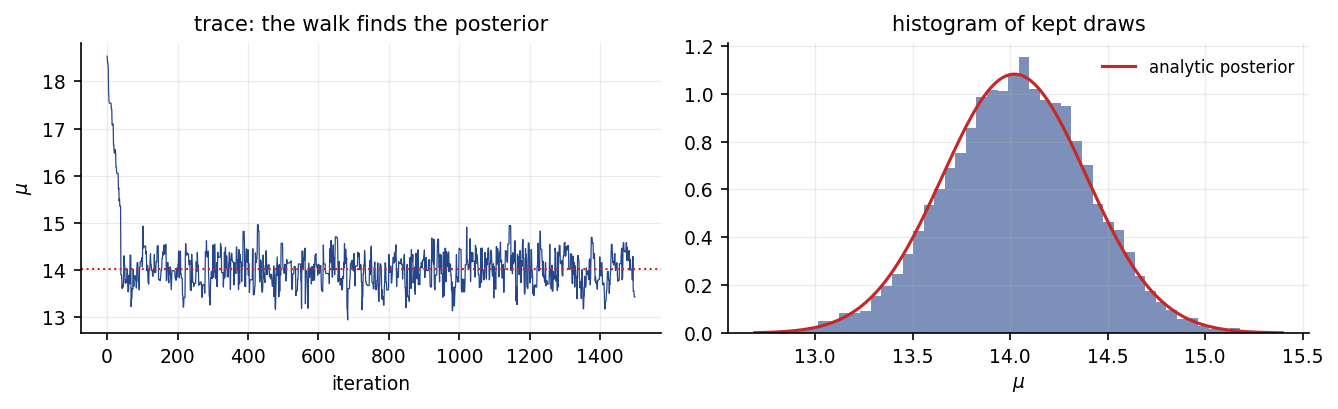
\includegraphics[width=0.9\textwidth,height=0.44\textheight,keepaspectratio]{cha12_metropolis.png}
  \end{center}
  \begin{numexample}[Sampler vs analytic truth]
    \footnotesize
    $20{,}000$ steps, acceptance rate $0.62$, burn-in $2{,}000$. Posterior mean
    $\mathbf{14.04}$ vs analytic $14.02$; posterior sd $\mathbf{0.367}$ vs analytic
    $0.369$. The trace (left) starts at a deliberately wrong value and finds the
    posterior within a few hundred steps.
  \end{numexample}
\end{frame}

\begin{frame}{Exercise A12.4 --- Reading a sampler [Concept]}
  \begin{exercise}
    Three colleagues run Metropolis on the same posterior and show you their
    diagnostics:
    \begin{enumerate}
      \item Colleague A: acceptance rate $0.99$; the trace drifts in slow waves.
      \item Colleague B: acceptance rate $0.02$; the trace is long flat plateaus.
      \item Colleague C: acceptance rate $0.55$; the trace is a fuzzy caterpillar.
    \end{enumerate}
    Diagnose each, name the shared root cause for A and B, and state the fix.
  \end{exercise}
\end{frame}

\begin{frame}{Solution --- Exercise A12.4}
  \begin{solutionbox}
    \footnotesize
    \textbf{A --- steps too small.} Nearly every proposal is accepted because it
    barely moves; the chain explores the posterior like a snail, and consecutive
    draws are almost copies. Estimates converge, but painfully slowly.
    \par\smallskip
    \textbf{B --- steps too large.} Proposals leap into low-probability territory
    and are almost always rejected; the chain freezes for hundreds of iterations.
    Same disease as A --- \emph{high autocorrelation in the chain} --- reached from
    the opposite direction.
    \par\smallskip
    \textbf{C --- healthy.} Mid-range acceptance with fast mixing; rules of thumb
    put the sweet spot around $0.2$--$0.5$ for random-walk Metropolis (our run:
    $0.62$, acceptably brisk for one dimension).
    \par\smallskip
    \textbf{Fix.} Tune the proposal scale $s$ toward the sweet spot; then confirm
    with the trace and by running a second chain from a different start and
    checking both agree.
  \end{solutionbox}
  \begin{mistake}
    Judging a sampler by acceptance rate alone. It is a symptom, not the disease:
    the disease is autocorrelation, and the trace plot (plus multiple chains) is
    the diagnostic that sees it.
  \end{mistake}
\end{frame}

\begin{frame}{Extended Exercise A12.1 --- Your own sampler [Python]}
  \begin{longexercise}
    Implement Metropolis from scratch for the mean of \texttt{Advertising} sales
    (treat $\sigma$ as the sample sd; prior $\mu \sim N(0, 100^2)$):
    \begin{enumerate}
      \item Write the log-posterior and the accept/reject loop; run $20{,}000$
            steps at proposal scale $0.5$ from the (bad) start $\bar x + 5$.
      \item Report acceptance rate, posterior mean and sd after burn-in; compare
            with the analytic values ($14.02$, $0.369$).
      \item Re-run with proposal scales $0.01$ and $50$. Connect what you see to
            Exercise A12.4.
    \end{enumerate}
  \end{longexercise}
\end{frame}

\begin{frame}[fragile]{Solution --- Extended Exercise A12.1 (1/2) --- code}
\begin{lstlisting}[basicstyle=\ttfamily\scriptsize]
import numpy as np, pandas as pd
x = pd.read_csv("Advertising.csv", index_col=0)["sales"].to_numpy()
rng = np.random.default_rng(2024)
sigma, tau, B, s = x.std(ddof=1), 100.0, 20_000, 0.5

def logpost(mu):                       # log posterior, up to a constant
    return -0.5*((x - mu)**2).sum()/sigma**2 - 0.5*mu**2/tau**2

chain, cur = np.empty(B), x.mean() + 5
lp = logpost(cur); acc = 0
for i in range(B):
    prop = cur + rng.normal(0, s)
    lp_prop = logpost(prop)
    if np.log(rng.uniform()) < lp_prop - lp:   # uphill: always; downhill: sometimes
        cur, lp, acc = prop, lp_prop, acc + 1
    chain[i] = cur
kept = chain[2000:]
print(f"accept {acc/B:.2f}, mean {kept.mean():.2f}, sd {kept.std(ddof=1):.3f}")
\end{lstlisting}
\end{frame}

\begin{frame}{Solution --- Extended Exercise A12.1 (2/2)}
  \begin{solutionbox}[Solution --- parts 2 and 3]
    \footnotesize
    \textbf{Part 2.} Acceptance $\approx 0.62$; posterior mean $14.04$, sd
    $0.367$ --- against analytic $14.02$ and $0.369$. A dozen lines of NumPy
    reproduce the exact answer to two decimals; that agreement \emph{is} the test
    that the sampler is correct.
    \par\smallskip
    \textbf{Part 3.} At $s = 0.01$ the acceptance rate rockets toward $1$ and the
    trace crawls (colleague A); at $s = 50$ acceptance collapses toward $0$ and
    the trace is plateaus (colleague B). Both chains still \emph{eventually}
    target the right posterior --- the theory guarantees the destination, tuning
    buys the arrival time.
  \end{solutionbox}
  \begin{mistake}
    Using $\pi(\theta')/\pi(\theta)$ on the raw (non-log) scale. With $n = 200$
    the likelihood underflows \texttt{float64} long before the ratio is formed ---
    always accept/reject on the \emph{log} scale, as the code does.
  \end{mistake}
\end{frame}

% ============================================================
\section{Regression \& Decisions}
% ============================================================

\begin{frame}{Bayesian simple regression: \texttt{sales} on \texttt{TV}}
  \begin{center}
    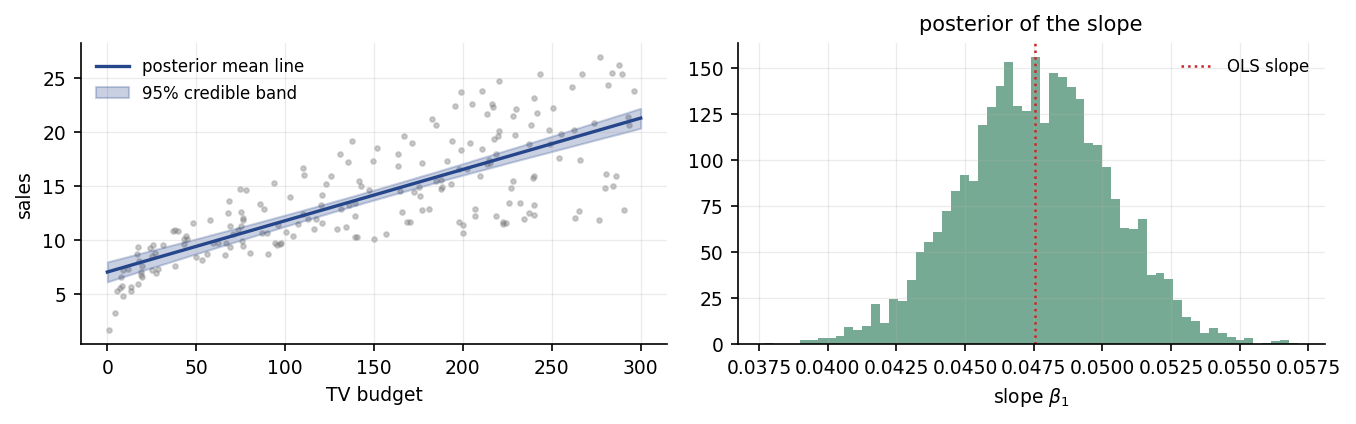
\includegraphics[width=0.76\textwidth,height=0.32\textheight,keepaspectratio]{cha12_bayes_reg.png}
  \end{center}
  \begin{numexample}[The posterior of a Chapter 3 slope]
    \footnotesize
    Weak $N(0, 10^2)$ priors on both coefficients. Posterior slope: mean
    $\mathbf{0.0476}$, sd $0.0027$ --- numerically the OLS fit ($0.0475$) with its
    standard error, \emph{reinterpreted}: the left panel's band is a $95\%$
    credible band of regression lines drawn from the posterior.
  \end{numexample}
  \begin{takeaway}[Weak priors reproduce Chapter 3 --- by design]
    \footnotesize
    With flat-ish priors, Bayesian regression rediscovers least squares; the
    machinery pays when priors carry information --- small $n$, correlated
    predictors (ridge!), hierarchies of related groups.
  \end{takeaway}
\end{frame}

\begin{frame}{A decision, not a $p$-value: the Bayesian A/B test}
  \begin{center}
    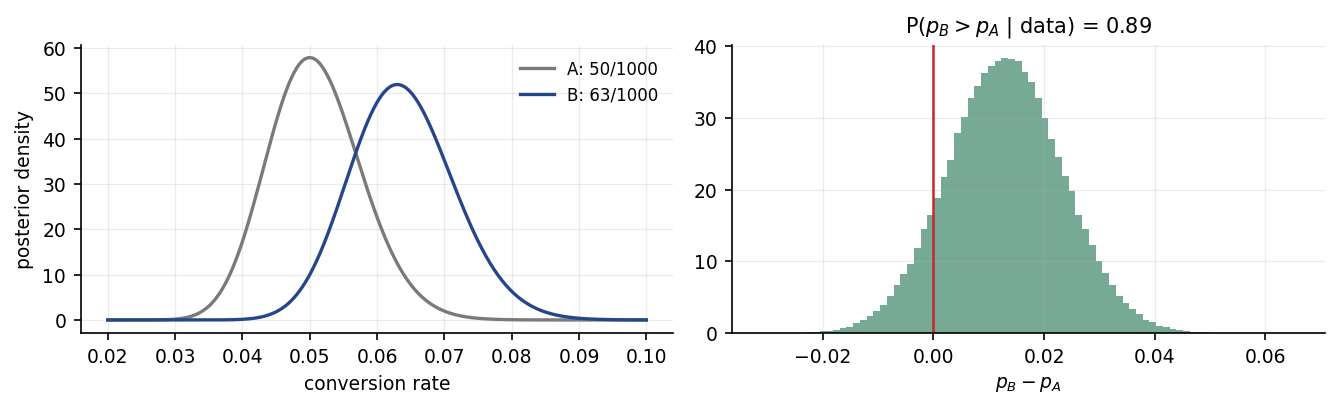
\includegraphics[width=0.8\textwidth,height=0.35\textheight,keepaspectratio]{cha12_ab.png}
  \end{center}
  \begin{numexample}[{{A: $50/1000$, B: $63/1000$}}]
    \footnotesize
    Flat priors, two independent Beta posteriors, $200{,}000$ paired draws:
    $\Pr(p_B > p_A \mid \text{data}) = \mathbf{0.895}$ --- a directly
    decision-shaped number. (The two-sided frequentist test at these counts does
    not clear $0.05$; both summaries are honest, they answer different questions.)
  \end{numexample}
  \begin{mistake}
    Believing posteriors are immune to module A1's peeking problem: if you
    \emph{stop when the posterior looks good}, the long-run error rate of that
    \emph{policy} still inflates --- design the stopping rule, whatever your
    school.
  \end{mistake}
\end{frame}

\begin{frame}{Extended Exercise A12.2 --- The Bayesian A/B memo [Integrative]}
  \begin{longexercise}
    Marketing ran the experiment above (A: $50/1000$, B: $63/1000$) and asks for a
    recommendation memo.
    \begin{enumerate}
      \item Reproduce $\Pr(p_B > p_A \mid \text{data})$ by simulation with flat
            priors. State the number with its meaning in one sentence.
      \item Compute the posterior of the \emph{lift} $p_B - p_A$ and report a
            $95\%$ credible interval. Does it contain $0$, and does that
            contradict part 1?
      \item Switching costs EUR~$2{,}000$; each conversion is worth EUR~$5$ on
            $100{,}000$ annual visitors. Turn the posterior into an expected-value
            decision.
      \item State one sentence of prior sensitivity: what would a sceptical prior
            (e.g.\ $\text{Beta}(50, 950)$ on both arms) do to the conclusion?
    \end{enumerate}
  \end{longexercise}
\end{frame}

\begin{frame}{Solution --- Extended Exercise A12.2}
  \begin{solutionbox}
    \footnotesize
    \textbf{Part 1.} Draw from $\text{Beta}(51, 951)$ and $\text{Beta}(64, 938)$,
    compare: $\Pr(p_B > p_A) \approx \mathbf{0.895}$ --- ``given the data, B is
    better with probability about $0.9$.''
    \par\smallskip
    \textbf{Part 2.} The lift's posterior is centred near $0.013$ with $95\%$ CrI
    roughly $[-0.007,\, 0.033]$ --- it \emph{does} straddle $0$. No contradiction:
    the CrI asks ``what values are plausible'', part 1 asks ``which arm is more
    likely better''; a $0.895$ direction is compatible with an interval touching
    zero.
    \par\smallskip
    \textbf{Part 3.} Expected lift $\approx 0.013 \times 100{,}000 \times$
    EUR~$5 = $ EUR~$6{,}500$/year against EUR~$2{,}000$ once; even weighting
    the downside draws, expected value favours switching --- recommend B, note the
    $\sim 10\%$ chance it is not better, and (module A1) confirm with a
    pre-registered follow-up if the cost were larger.
    \par\smallskip
    \textbf{Part 4.} A sceptical $\text{Beta}(50, 950)$ prior (five percent, held
    with $1000$ trials' conviction) roughly halves the estimated lift and pulls
    $\Pr(p_B > p_A)$ toward $0.8$ --- the direction survives, the enthusiasm
    moderates. Report both runs.
  \end{solutionbox}
\end{frame}

% ============================================================
\section{Python Lab}
% ============================================================

\begin{frame}{Python lab --- run it live}
  \begin{labnote}[{{Reproduce every number: \texttt{make\_figures.py}}}]
    Every number on these slides is computed by \texttt{make\_figures.py} in this
    module's folder, from the bundled \texttt{Advertising.csv} and seeded
    simulations --- run it and read it alongside the deck:
    \begin{itemize}
      \item the Beta--binomial updates ($\text{Beta}(2,2) \to \text{Beta}(51,153)$)
            and the three-priors picture;
      \item the precision-weighted Gaussian posteriors ($w = 0.53 \to 0.97$);
      \item the from-scratch Metropolis run ($14.04$ vs analytic $14.02$);
      \item Bayesian regression on \texttt{Advertising} and the ridge--MAP dial;
      \item the A/B posterior ($\Pr(p_B > p_A) = 0.895$).
    \end{itemize}
    A companion notebook in the course lab format is in preparation; until it
    lands, the script \emph{is} the lab --- it runs top to bottom in the course
    environment with no extra packages.
  \end{labnote}
\end{frame}

\begin{frame}[fragile]{The whole module in twelve lines}
\begin{lstlisting}
import numpy as np
from scipy import stats
rng = np.random.default_rng(2024)

# belief -> data -> updated belief, all in one conjugate line
a, b = 2, 2                       # prior Beta(2,2): four imaginary trials
y, n = 49, 200                    # the data
post = stats.beta(a + y, b + n - y)
print(f"posterior mean {post.mean():.3f}, "
      f"95% CrI [{post.ppf(0.025):.3f}, {post.ppf(0.975):.3f}]")

# and the sentence the frequentist interval cannot say:
print(f"P(p > 0.25 | data) = {1 - post.cdf(0.25):.2f}")
\end{lstlisting}
\end{frame}

% ============================================================
\section{Summary}
% ============================================================

\begin{frame}{Module A12 in one slide}
  \begin{block}{What we accomplished}
    A second, coherent grammar for uncertainty --- run on the course's own
    likelihoods and datasets.
  \end{block}
  \begin{itemize}
    \item Posterior $\propto$ likelihood $\times$ prior --- Chapter 4's theorem,
          aimed at parameters.
    \item Beta--binomial updating by hand: $\text{Beta}(2,2)$ plus $200$ trials
          $\to \text{Beta}(51,153)$, CrI $[0.193, 0.312]$.
    \item Every posterior mean is a precision-weighted compromise; the data's
          weight grows as $n / (n + \text{imaginary } n)$.
    \item Ridge unmasked: MAP under $N(0, \tau^2)$ priors, $\lambda =
          \sigma^2/\tau^2$ --- Chapter 6 was Bayesian all along.
    \item Metropolis from scratch: $14.04 \pm 0.367$ against analytic
          $14.02 \pm 0.369$.
    \item Decision-shaped output: $\Pr(p_B > p_A \mid \text{data}) = 0.895$ ---
          with the peeking caveat imported from A1.
  \end{itemize}
\end{frame}

\begin{frame}{Key formulas at a glance}
  \footnotesize
  \begin{description}
    \item[Bayes for parameters] $\pi(\theta \mid \text{data}) \propto
      L(\theta)\,\pi(\theta)$.
    \item[Beta--binomial] $\text{Beta}(a,b) + (y, n) \to
      \text{Beta}(a{+}y,\, b{+}n{-}y)$; mean $(a{+}y)/(a{+}b{+}n)$.
    \item[Shrinkage weight] posterior mean $= w\,\hat\theta_{\text{data}} +
      (1{-}w)\,\theta_{\text{prior}}$, $w = n/(n + a + b)$ (Beta) or
      $\frac{n/\sigma^2}{n/\sigma^2 + 1/\tau^2}$ (Gaussian).
    \item[Gaussian posterior] precision $= n/\sigma^2 + 1/\tau^2$; precisions add,
      never sds.
    \item[Ridge as MAP] $\hat\beta_{\text{ridge}} = \arg\max$ posterior under
      $\beta_j \sim N(0, \tau^2)$, with $\lambda = \sigma^2/\tau^2$.
    \item[Metropolis] accept $\theta'$ w.p.\ $\min\{1,
      \pi(\theta'\mid\text{data})/\pi(\theta\mid\text{data})\}$ --- ratios only,
      log scale in code.
  \end{description}
\end{frame}

\begin{frame}{Vocabulary checklist}
  \footnotesize
  \begin{center}
  \begin{tabular}{@{}ll@{}}
    \toprule
    \textbf{Term} & \textbf{Meaning} \\
    \midrule
    prior & belief about $\theta$ before the data, as a distribution \\
    likelihood & $p(\text{data} \mid \theta)$ --- Chapters 3--4's fit criterion \\
    posterior & updated belief; the module's universal output \\
    conjugate prior & family the posterior stays inside (Beta for binomial) \\
    credible interval & interval holding stated posterior probability \\
    MAP & posterior mode; ridge and lasso are MAPs \\
    shrinkage & posterior pulled from data toward prior \\
    burn-in & discarded warm-up of an MCMC chain \\
    acceptance rate & share of Metropolis proposals taken; tune toward mid-range \\
    prior sensitivity & re-running with other priors; always reported \\
    \bottomrule
  \end{tabular}
  \end{center}
\end{frame}

\begin{frame}{Decision rules of thumb}
  \begin{itemize}
    \item Small $n$, real prior knowledge, or a decision to make $\Rightarrow$
          Bayesian machinery earns its keep. Large $n$, flat priors $\Rightarrow$
          it will agree with Chapter 0; use whichever is cheaper.
    \item Choose priors you can defend out loud, in units of imaginary
          observations --- and always show a sensitivity run.
    \item Report the whole posterior (or its CrI), not just a point; say
          \emph{which} point if you must give one.
    \item Conjugate first, grid second, MCMC when you must; always check a sampler
          against a case with a known answer.
    \item Trace plot + second chain before trusting any MCMC number.
    \item Probability statements about parameters: credible intervals only ---
          never launder a confidence interval into one.
  \end{itemize}
\end{frame}

\begin{frame}{Common pitfalls}
  \begin{alertblock}{Don't}
    \begin{enumerate}
      \item Read a confidence interval as ``$95\%$ probability the parameter is
            inside'' --- that sentence needs a posterior.
      \item Hide an informative prior ($\text{Beta}(30,10)$ moved the answer from
            $0.32$ to $0.60$ on the same data).
      \item Add standard deviations where only precisions add.
      \item Compute likelihood ratios off the log scale ($n = 200$ already
            underflows).
      \item Trust a chain by its acceptance rate alone --- plateaus and snails
            both lie.
      \item Peek-and-stop on a posterior and claim the error rate of a fixed-$n$
            design.
    \end{enumerate}
  \end{alertblock}
\end{frame}

\begin{frame}{Self-check questions}
  \scriptsize
  \begin{readme}[{{Quick self-assessment}}]
    \begin{enumerate}
      \item Prior $\text{Beta}(2,2)$, then $7$ successes in $10$ trials: posterior,
            posterior mean, and the weight on the data?
      \item Prior $N(100, 15^2)$, $\sigma = 20$, $n = 4$, $\bar x = 120$: posterior
            mean?
      \item State the ridge--Bayes dictionary in one equation.
      \item Your Metropolis run has acceptance $0.99$ and a slowly drifting trace.
            Diagnosis and fix?
      \item $\Pr(p_B > p_A \mid \text{data}) = 0.895$ while the $95\%$ CrI for
            $p_B - p_A$ includes $0$. Contradiction?
      \item What is the one sentence a credible interval may say that a confidence
            interval may not?
    \end{enumerate}
  \end{readme}
  \begin{takeaway}[{{Answers}}]
    (1) $\text{Beta}(9,5)$; $9/14 \approx 0.643$; $w = 10/14 \approx 0.71$.
    (2) $w \approx 0.69$, mean $\approx 113.8$. (3) $\lambda = \sigma^2/\tau^2$
    under $\beta_j \sim N(0, \tau^2)$. (4) Proposal scale too small --- enlarge
    $s$ toward acceptance $\sim 0.2$--$0.5$, confirm on the trace. (5) No: one is
    a statement about direction, the other about plausible magnitudes; both are
    read off the same posterior. (6) ``Given the data, the parameter lies in this
    interval with probability $0.95$.''
  \end{takeaway}
\end{frame}

\begin{frame}{Five things to remember}
  \begin{takeaway}[Module A12 in five lines]
    \begin{enumerate}
      \item \textbf{Posterior $\propto$ likelihood $\times$ prior} --- one line,
            the whole framework.
      \item \textbf{Every estimate is a compromise weighted by precision} --- the
            data's weight is $n$ against the prior's imaginary $n$.
      \item \textbf{Ridge is a prior in disguise:} $\lambda = \sigma^2/\tau^2$ ---
            Chapter 6 has been Bayesian all along.
      \item \textbf{MCMC trades formulas for a walk} --- and a from-scratch
            Metropolis matched the analytic answer to two decimals.
      \item \textbf{Priors are claims with stakes:} state them, price them in
            imaginary trials, and show the sensitivity run.
    \end{enumerate}
  \end{takeaway}
\end{frame}

\begin{frame}{What's next}
  \begin{itemize}
    \item \textbf{Module A1 --- Randomised Controlled Trials}: the A/B decision
          slide is A1's experiment wearing posterior clothes --- and A1's peeking
          warning survives the change of school.
    \item \textbf{Chapter 6, re-read}: the ridge and lasso paths are prior
          strength dialled from $\infty$ to $0$; the Bayesian reading explains
          \emph{why} shrinking helps when $p$ is large.
    \item \textbf{Module A3 --- Conformal Prediction}: the frequentist route to
          calibrated uncertainty --- guarantees without priors, at the price of
          answering only about \emph{predictions}. Reading A3 and A12 together
          maps the whole uncertainty landscape.
  \end{itemize}
\end{frame}

% ============================================================
\appendix
\AtBeginSection[]{}
\section{Appendix: optional and advanced material}
% ============================================================

\begin{frame}{Appendix --- what is in here, and why}
  \footnotesize
  Nothing in the appendix is needed to follow the module: each slide is a formal
  derivation, a longer worked exercise, or a side topic. Read it when you want the
  full story, or when a later chapter sends you back here.
  \begin{block}{Contents of the appendix}
    \begin{itemize}
      \item \textbf{The Beta--binomial update, derived} --- two lines of algebra;
            moved out because the recipe, not the proof, carries the deck.
      \item \textbf{A conjugate-pairs reference table} --- look-up material.
      \item \textbf{The posterior predictive} --- forecasting a new observation,
            not a parameter; the bridge to Chapters 3 and A3.
    \end{itemize}
  \end{block}
\end{frame}

\begin{frame}{The Beta--binomial update, derived}
  \footnotesize
  Prior density $\pi(p) \propto p^{a-1}(1-p)^{b-1}$; binomial likelihood
  $L(p) \propto p^{y}(1-p)^{n-y}$. Multiply:
  \[
    \pi(p \mid y) \;\propto\; p^{y}(1-p)^{n-y} \cdot p^{a-1}(1-p)^{b-1}
    \;=\; p^{(a+y)-1}\,(1-p)^{(b+n-y)-1},
  \]
  which is the kernel of $\text{Beta}(a+y,\; b+n-y)$ --- no integral was ever
  computed; recognising the \emph{shape} suffices.
  \begin{takeaway}[Why conjugacy is a big deal]
    The prior and posterior live in the same family, so updating is arithmetic on
    two counters $(a, b)$ --- streaming data update beliefs in $O(1)$, and the
    ``imaginary trials'' reading of the prior is literal.
  \end{takeaway}
\end{frame}

\begin{frame}{Conjugate pairs at a glance}
  \footnotesize
  \begin{center}
  \begin{tabular}{@{}lll@{}}
    \toprule
    \textbf{Likelihood} & \textbf{Conjugate prior} & \textbf{Posterior update} \\
    \midrule
    Binomial $(n, p)$ & $\text{Beta}(a, b)$ & $a{+}y$, $b{+}n{-}y$ \\
    Poisson $(\lambda)$ & $\text{Gamma}(a, b)$ & $a + \textstyle\sum y_i$, $b + n$ \\
    Gaussian mean (known $\sigma$) & $N(\mu_0, \tau^2)$ & precision-weighted
      (main deck) \\
    Gaussian variance (known $\mu$) & Inverse-Gamma & shape ${+}\,n/2$ \\
    Multinomial & Dirichlet & add the category counts \\
    \bottomrule
  \end{tabular}
  \end{center}
  \begin{readme}[How to use this table]
    Each row is the same story: the prior is phrased as pseudo-data, and updating
    adds real data to it. Module A4's exponential-family machinery is the deep
    reason this table exists: every exponential-family likelihood has a conjugate
    family of exactly this form.
  \end{readme}
\end{frame}

\begin{frame}{The posterior predictive: betting on the next observation}
  \footnotesize
  For a new observation $\tilde y$, integrate predictions over the posterior:
  \[
    p(\tilde y \mid \text{data})
      = \int p(\tilde y \mid \theta)\,\pi(\theta \mid \text{data})\, d\theta .
  \]
  \begin{numexample}[The next conversion]
    After $\text{Beta}(51, 153)$: $\Pr(\tilde y = 1 \mid \text{data}) =
    E[p \mid \text{data}] = 51/204 = 0.25$ --- but for the next \emph{twenty}
    visitors the predictive is Beta-binomial, \emph{wider} than
    $\text{Binomial}(20, 0.25)$, because parameter uncertainty rides along.
  \end{numexample}
  \begin{takeaway}[The bridge to prediction intervals]
    Chapter 3's prediction intervals and module A3's conformal sets solve this
    same problem in frequentist dress: honest forecasts must carry \emph{both}
    noise and parameter uncertainty. The posterior predictive is the Bayesian
    statement of that requirement.
  \end{takeaway}
\end{frame}

\end{document}
